\documentclass[a4paper,german,12pt,smallheadings]{scrartcl}
\usepackage[T1]{fontenc}
\usepackage[utf8]{inputenc}
\usepackage{babel}
\usepackage{tikz}
\usetikzlibrary{calc}
\usepackage{tkz-euclide}
\usetkzobj{all}
\usepackage{pgfplots}
\usepackage{geometry}
\usepackage{longtable}
\usepackage[fleqn]{amsmath}
\usepackage{amssymb}
\usepackage{float}
\usepackage{lscape}
\usepackage{enumerate}
\usepackage{commath} % http://tex.stackexchange.com/questions/14821/whats-the-proper-way-to-typeset-a-differential-operator
\usepackage{cancel}
\usepackage{gnuplottex}

% Number only referenced equations
\usepackage[fleqn]{mathtools}
\mathtoolsset{showonlyrefs}

%\usepackage{wrapfig}
\usepackage{siunitx}
\sisetup{locale = DE}

% New command for color underlining
\usepackage{xcolor}

\newsavebox\MBox
\newcommand\colul[2][red]{{\sbox\MBox{$#2$}%
  \rlap{\usebox\MBox}\color{#1}\rule[-1.2\dp\MBox]{\wd\MBox}{0.5pt}}}

% Stupid units for astronomy
\DeclareSIUnit\day{d}
\DeclareSIUnit\year{yr}
\DeclareSIUnit\au{AU}
% Astronomy-Style angles (hours, minutes, seconds)
\newcommand*{\ra}[2][]{{
  \def\SIUnitSymbolDegree{\textsuperscript{h}}%
  \def\SIUnitSymbolArcminute{\textsuperscript{m}}%
  \def\SIUnitSymbolArcsecond{\textsuperscript{s}}%
  \ang[#1]{#2}}%
}

\restylefloat{table}
\geometry{a4paper, top=15mm, left=10mm, right=20mm, bottom=20mm, headsep=10mm, footskip=12mm}
\linespread{1.2}
\setlength\parindent{0pt}
\DeclareMathOperator{\Tr}{Tr}
\DeclareMathOperator{\Var}{Var}

\begin{document}
\allowdisplaybreaks % Seitenumbrüche in Formeln erlauben
\begin{center}
\bfseries % Fettdruck einschalten
\sffamily % Serifenlose Schrift
\vspace{-40pt}
Einführung in die Astronomie und Astrophysik, Sommersemester 2014, Aufgabenblatt 9

Markus Fenske, Julia Schuch, Tutor: Daniel Härdt
\vspace{-10pt}
\end{center}
\section*{Aufgabe 1: Fleißaufgabe ohne Lerneffekt}
\begin{enumerate}[a)]
  \item
    Die kinetische Energie der Kugelsternhaufen ist (unter Vernachlässigung interner kinetischer Energie)
    \begin{equation}
      E_\text{kin} = \frac{1}{2} m v^2.
    \end{equation}

    Die potentielle Energie ist (unter Vernachlässigung jeglicher Interaktion
    untereinander und der Annahe einer sphärischen Milchstraße)
    \begin{equation}
      E_\text{pot} = \frac{GM(r)m}{r}
    \end{equation}

    Unter Nutzung des Virialsatzes
    \begin{equation}
      \left<E_\text{pot}\right> + 2 \left<E_\text{kin}\right> = 0
    \end{equation}

    und der Annahme, dass die momentanen Geschwindigkeiten ihren Mittelwerten
    entsprechen, erhalten wir
    \begin{equation}
      1 = -\frac{2\sum E_\text{kin}}{\sum E_\text{pot}} = \frac{\sum m_i v_i^2}{\sum \dfrac{GM m_i}{r_i}}
    \end{equation}

    Umstellen und Vernachlässigung der kinetischen Energie der Milchstraße
    ergibt
    \begin{equation}
      M = \frac{\sum m_i v_i^2}{G \sum \dfrac{m_i}{R_i}}
    \end{equation}

    Wenn wir annehmen, dass die Massen aller Kugelsternhaufen gleich sind und
    dass die Kugelsternhaufen sphärisch verteilt sind, so dass die
    Geschwindigkeitsquadrate durch die Radialgeschwindigkeiten ausgedrückt
    werden können: $v_i^2 = 3 u_i^2$, erhalten wir
    \begin{equation}
      M = \frac{3 \sum u_i^2}{G \sum \frac{1}{R_i}}
    \end{equation}
  \item Mit der Gleichung aus a) ergeben sich folgende Werte:

    \begin{longtable}{|l|l|l|l|l|l|}
    \hline
    $k$  & NGC Nr. &R [kpc] & $u$ [km/s] & $\sum_{i=1}^k R_i^{-1}$
    [$\mathrm{kpc}^-1$] & $M(k)$ [$M_\odot$] \\
     1 & 2419 & $\num{77.1}$ & -4   & $\num{0.0013}$ & $\num{1.8e9}$ \\
     2 & 5694 & $\num{45.3}$ & -281 & $\num{0.0036}$ & $\num{572e9}$ \\
     3 & 7006 & $\num{43.5}$ & -109 & $\num{0.0060}$ & $\num{092e9}$ \\
     4 & 2298 & $\num{26.5}$ & -187 & $\num{0.0100}$ & $\num{916e9}$ \\
     5 & 6229 & $\num{24.8}$ & 63   & $\num{0.0142}$ & $\num{665e9}$ \\
     6 & 4147 & $\num{24,1}$ & 1    & $\num{0.0186}$ & $\num{587e9}$ \\
     7 & 1904 & $\num{22.9}$ & 36   & $\num{0.0232}$ & $\num{475e9}$ \\
     8 & 5824 & $\num{20.9}$ & -156 & $\num{0.0282}$ & $\num{454e9}$ \\
     9 & 5024 & $\num{19.6}$ & -120 & $\num{0.0336}$ & $\num{413e9}$ \\
    10 & 1851 & $\num{18.3}$ & 76   & $\num{0.0393}$ & $\num{363e9}$ \\
    11 & 5634 & $\num{17.4}$ & -96  & $\num{0.0454}$ & $\num{330e9}$ \\
    12 & 6864 & $\num{15.4}$ & -122 & $\num{0.0522}$ & $\num{308e9}$ \\
    13 & 6981 & $\num{14.9}$ & -113 & $\num{0.0592}$ & $\num{287e9}$ \\
    14 & 6934 & $\num{13.9}$ & -146 & $\num{0.0668}$ & $\num{278e9}$ \\
    15 & 7089 & $\num{13.3}$ & 181  & $\num{0.0747}$ & $\num{280e9}$ \\
    16 & 6779 & $\num{12.9}$ & 98   & $\num{0.0828}$ & $\num{261e9}$ \\
    17 & 7078 & $\num{12.4}$ & 111  & $\num{0.0913}$ & $\num{247e9}$ \\
    18 & 5272 & $\num{12.0}$ & -100 & $\num{0.1000}$ & $\num{233e9}$ \\
    19 & 6681 & $\num{11.5}$ & 229  & $\num{0.1092}$ & $\num{248e9}$ \\
    20 & 6341 & $\num{11.1}$ & 103  & $\num{0.1186}$ & $\num{235e9}$ \\
    21 & 4590 & $\num{10.8}$ & -292 & $\num{0.1284}$ & $\num{266e9}$ \\
    22 & 7099 & $\num{10.0}$ & -72  & $\num{0.1389}$ & $\num{248e9}$ \\
    23 & 6205 & $\num{ 9.0}$ & -36  & $\num{0.1505}$ & $\num{230e9}$ \\
    24 & 6284 & $\num{ 8.6}$ & 37   & $\num{0.1628}$ & $\num{213e9}$ \\
    25 & 6652 & $\num{ 7.4}$ & -98  & $\num{0.1769}$ & $\num{200e9}$ \\
    26 & 5986 & $\num{ 7.2}$ & -79  & $\num{0.1915}$ & $\num{187e9}$ \\
    27 & 5904 & $\num{ 7.1}$ & 80   & $\num{0.2063}$ & $\num{176e9}$ \\
    28 & 6171 & $\num{ 6.7}$ & -109 & $\num{0.2220}$ & $\num{167e9}$ \\
    29 & 6440 & $\num{ 6.5}$ & -76  & $\num{0.2382}$ & $\num{158e9}$ \\
    30 & 6638 & $\num{ 6.2}$ & 46   & $\num{0.2551}$ & $\num{148e9}$ \\
    31 & 6656 & $\num{ 6.2}$ & -83  & $\num{0.2720}$ & $\num{140e9}$ \\
    32 & 6626 & $\num{ 5.2}$ & 57   & $\num{0.2922}$ & $\num{132e9}$ \\
    33 & 6218 & $\num{ 5.0}$ & 124  & $\num{0.3132}$ & $\num{126e9}$ \\
    34 & 6293 & $\num{ 5.0}$ & -63  & $\num{0.3342}$ & $\num{119e9}$ \\
    35 & 6254 & $\num{ 4.9}$ & 163  & $\num{0.3557}$ & $\num{117e9}$ \\
    36 & 6402 & $\num{ 4.4}$ & -12  & $\num{0.3795}$ & $\num{110e9}$ \\
    37 & 6712 & $\num{ 4.3}$ & 5    & $\num{0.4040}$ & $\num{103e9}$ \\
    38 & 6304 & $\num{ 4.2}$ & -93  & $\num{0.4290}$ & $\num{ 99e9}$ \\
    39 & 6723 & $\num{ 3.6}$ & 17   & $\num{0.4581}$ & $\num{ 93e9}$ \\
    40 & 6624 & $\num{ 3.5}$ & 101  & $\num{0.4882}$ & $\num{ 88e9}$ \\
    41 & 6093 & $\num{ 3.4}$ & 11   & $\num{0.5190}$ & $\num{ 83e9}$ \\
    42 & 6273 & $\num{ 3.4}$ & 112  & $\num{0.5499}$ & $\num{ 80e9}$ \\
    43 & 6637 & $\num{ 3.4}$ & 122  & $\num{0.5808}$ & $\num{ 78e9}$ \\
    44 & 6715 & $\num{ 3.4}$ & 151  & $\num{0.6117}$ & $\num{ 76e9}$ \\
    45 & 6333 & $\num{ 3.1}$ & 272  & $\num{0.6456}$ & $\num{ 81e9}$ \\
    46 & 6266 & $\num{ 2.9}$ & -90  & $\num{0.6818}$ & $\num{ 77e9}$ \\
    47 & 6356 & $\num{ 2.3}$ & 84   & $\num{0.7275}$ & $\num{ 73e9}$ \\
    48 & 6441 & $\num{ 2.3}$ & -80  & $\num{0.7731}$ & $\num{ 69e9}$ \\
    \hline
    \end{longtable}

  \item
    Plot siehe letzte Seite. Aus dem Plot erhalten wir
    \begin{equation}
    M(1/R) = \frac{a}{1/R} \text{ mit } a = \num{2.146+-0.037} \cdot 10^{10} \mathrm{kpc} M_\odot
    \end{equation}

    bei $R = \SI{100}{kpc}$ ergibt sich also eine Masse
    \begin{equation}
      M_{100} = 2{,}146 \cdot 10^{12} M_\odot
    \end{equation}
  \item
    Die berechnete Masse beträgt etwa 71\% des Literaturwerts. Dies ist in den
    vielen Näherungen begründet. Daraus einen Einfluss dunkler Materie erkennen
    zu wollen ist Unfug.

    % Trolling :)
    Dunkle Materie wurde bis jetzt nicht nachgewiesen. Die Rotationsanomalie
    und die Strukturierung des Universums lassen sich hervorragend mithilfe
    einer Quantengravitationstheorie erklären. Dabei muss einerseits die
    Gravitationswirkung des Gravitationsfeldes als Energie- und Impulsträger
    selber und damit seine Selbstinteraktion berücksichtig werden, andererseits
    muss beachtet werden, dass die Wellenlänge der Gravitonen von der
    Massenzahl der verursachenden Elemente abhängt, so dass sich für
    unterschiedlich zusammengesetzte Körper unterschiedliche Wellenlängen
    ergeben. Die Wellenlänge liegt dabei in kosmologischen Bereichen, so dass
    die Quanteneffekte erst dort sichtbar werden. In Sonnensystemgrenzen gilt
    in sehr guter Näherung die klassische Theorie, so dass diese Effekte bis
    jetzt nicht bemerkt wurden, außer von der Pioneer-Sonde, was jedoch auf
    eine anisotrope Wärmeabstrahlung der Sonde zurückgeführt wird.

  \item
    Aus dem 3. Keplerschen Gesetz
    \begin{equation}
      \frac{a^3}{T^2} \approx \frac{4 \pi^2}{GM}
    \end{equation}

    folgt mit der Umlaufdauer
    \begin{equation}
      T = 2 \pi \frac{a}{v}
    \end{equation}

    die Masse
    \begin{equation}
      M = \frac{a v^2}{G} = 1{,}027 \cdot 10^{11} M_\odot
    \end{equation}

    Mit $M(R) = \frac{a}{R}$ und $M(8 kpc) = 1{,}027 \cdot 10^{11} M_\odot$ ergibt sich
    \begin{equation}
      a = 8{,}216 \cdot 10^{11} M_\odot
    \end{equation}

    Was mit der selben Extrapolation wie in c) auf folgende Masse führt:
    \begin{equation}
      M_{100} = 8{,}216 \cdot 10^{13} M_\odot
    \end{equation}

    Diese liegt viel höher als das selbe Ergebnis, was darin liegt, dass mit
    der Fitgleichung angenommen wird, dass die Milchstraße eine homogene
    Massenverteilung hat. Dies ist nicht der Fall. Die Sonne befindet sich in
    einem dichteren Teil der Milchstraße als die Kugelsternhaufen.

  \item
    Darin sehe ich keinen Sinn. Man müsste zuerst die ganzen Näherungen durch
    anständige Annahmen ersetzen, bevor man daraus irgendeine
    Massenzusammensetzung erkennen möchte.
\end{enumerate}

\section*{Aufgabe 3: Potentielle Energie einer Molekülwolke}
Die potentielle Energie ist die Energie, die ich erhalte, wenn ich die Wolke
zusammenbaue.

Angenommen es gäbe bereits eine kugelförmige Masse $M$ und ich hole aus
unendlicher Entfernung eine kleine Masse $dM$ die ich sphärisch um die Kugel
verteile, dann wird die potentielle Energie
\begin{equation}
  dV = - \frac{G M dM}{r}
\end{equation}
frei.

Wenn ich die Wolke aus solchen sphärischen Schichten der Dichte $\rho$ aufbaue,
erhalte ich jeweils eine zusätzliche Kugelschale der Dichte $\rho$ mit dem
Radius $dr$. Diese hat jeweils die Masse
\begin{equation}
  dM = 4 \pi r^2 \rho dr
\end{equation}

Angenommen, ich habe solche Schichten bis zum Radius $r$ gestapelt und die
Dichte sei konstant, dann ist die Masse
\begin{equation}
  M(r) = \rho V = \rho \frac{4}{3} \pi r^3
\end{equation}

Wenn wir über die einzelnen Schichten integrieren, erhalten wir
\begin{equation}
  V = -G \int_0^R \frac{M(r) dM(r)}{r} = -G \frac{16 \pi^2}{4} \rho^2 \int_0^R \dif \; r^4 = -G\frac{16 \pi^2 \rho^2}{4} \frac{1}{5} R^5
\end{equation}

Mit
\begin{equation}
  \rho = \frac{M}{V} = \frac{3 M}{4 \pi R^3}
\end{equation}

also
\begin{equation}
  V = -G \frac{16 \pi^2}{4} \frac{1}{5} R^5 \frac{9 M^2}{16\pi^2 R^6} = - \frac{3}{5} \frac{G M^2}{R}
\end{equation}

\newpage
\begin{landscape}
  % gnuplot ./data-9.gnuplot
  % GNUPLOT: LaTeX picture with Postscript
\begingroup
  \makeatletter
  \providecommand\color[2][]{%
    \GenericError{(gnuplot) \space\space\space\@spaces}{%
      Package color not loaded in conjunction with
      terminal option `colourtext'%
    }{See the gnuplot documentation for explanation.%
    }{Either use 'blacktext' in gnuplot or load the package
      color.sty in LaTeX.}%
    \renewcommand\color[2][]{}%
  }%
  \providecommand\includegraphics[2][]{%
    \GenericError{(gnuplot) \space\space\space\@spaces}{%
      Package graphicx or graphics not loaded%
    }{See the gnuplot documentation for explanation.%
    }{The gnuplot epslatex terminal needs graphicx.sty or graphics.sty.}%
    \renewcommand\includegraphics[2][]{}%
  }%
  \providecommand\rotatebox[2]{#2}%
  \@ifundefined{ifGPcolor}{%
    \newif\ifGPcolor
    \GPcolorfalse
  }{}%
  \@ifundefined{ifGPblacktext}{%
    \newif\ifGPblacktext
    \GPblacktexttrue
  }{}%
  % define a \g@addto@macro without @ in the name:
  \let\gplgaddtomacro\g@addto@macro
  % define empty templates for all commands taking text:
  \gdef\gplbacktext{}%
  \gdef\gplfronttext{}%
  \makeatother
  \ifGPblacktext
    % no textcolor at all
    \def\colorrgb#1{}%
    \def\colorgray#1{}%
  \else
    % gray or color?
    \ifGPcolor
      \def\colorrgb#1{\color[rgb]{#1}}%
      \def\colorgray#1{\color[gray]{#1}}%
      \expandafter\def\csname LTw\endcsname{\color{white}}%
      \expandafter\def\csname LTb\endcsname{\color{black}}%
      \expandafter\def\csname LTa\endcsname{\color{black}}%
      \expandafter\def\csname LT0\endcsname{\color[rgb]{1,0,0}}%
      \expandafter\def\csname LT1\endcsname{\color[rgb]{0,1,0}}%
      \expandafter\def\csname LT2\endcsname{\color[rgb]{0,0,1}}%
      \expandafter\def\csname LT3\endcsname{\color[rgb]{1,0,1}}%
      \expandafter\def\csname LT4\endcsname{\color[rgb]{0,1,1}}%
      \expandafter\def\csname LT5\endcsname{\color[rgb]{1,1,0}}%
      \expandafter\def\csname LT6\endcsname{\color[rgb]{0,0,0}}%
      \expandafter\def\csname LT7\endcsname{\color[rgb]{1,0.3,0}}%
      \expandafter\def\csname LT8\endcsname{\color[rgb]{0.5,0.5,0.5}}%
    \else
      % gray
      \def\colorrgb#1{\color{black}}%
      \def\colorgray#1{\color[gray]{#1}}%
      \expandafter\def\csname LTw\endcsname{\color{white}}%
      \expandafter\def\csname LTb\endcsname{\color{black}}%
      \expandafter\def\csname LTa\endcsname{\color{black}}%
      \expandafter\def\csname LT0\endcsname{\color{black}}%
      \expandafter\def\csname LT1\endcsname{\color{black}}%
      \expandafter\def\csname LT2\endcsname{\color{black}}%
      \expandafter\def\csname LT3\endcsname{\color{black}}%
      \expandafter\def\csname LT4\endcsname{\color{black}}%
      \expandafter\def\csname LT5\endcsname{\color{black}}%
      \expandafter\def\csname LT6\endcsname{\color{black}}%
      \expandafter\def\csname LT7\endcsname{\color{black}}%
      \expandafter\def\csname LT8\endcsname{\color{black}}%
    \fi
  \fi
  \setlength{\unitlength}{0.0500bp}%
  \begin{picture}(15306.00,10204.00)%
    \gplgaddtomacro\gplbacktext{%
      \csname LTb\endcsname%
      \put(1474,704){\makebox(0,0)[r]{\strut{} 0}}%
      \put(1474,1730){\makebox(0,0)[r]{\strut{} 5e+10}}%
      \put(1474,2756){\makebox(0,0)[r]{\strut{} 1e+11}}%
      \put(1474,3782){\makebox(0,0)[r]{\strut{} 1.5e+11}}%
      \put(1474,4808){\makebox(0,0)[r]{\strut{} 2e+11}}%
      \put(1474,5835){\makebox(0,0)[r]{\strut{} 2.5e+11}}%
      \put(1474,6861){\makebox(0,0)[r]{\strut{} 3e+11}}%
      \put(1474,7887){\makebox(0,0)[r]{\strut{} 3.5e+11}}%
      \put(1474,8913){\makebox(0,0)[r]{\strut{} 4e+11}}%
      \put(1474,9939){\makebox(0,0)[r]{\strut{} 4.5e+11}}%
      \put(1606,484){\makebox(0,0){\strut{} 0.05}}%
      \put(3269,484){\makebox(0,0){\strut{} 0.1}}%
      \put(4932,484){\makebox(0,0){\strut{} 0.15}}%
      \put(6595,484){\makebox(0,0){\strut{} 0.2}}%
      \put(8258,484){\makebox(0,0){\strut{} 0.25}}%
      \put(9920,484){\makebox(0,0){\strut{} 0.3}}%
      \put(11583,484){\makebox(0,0){\strut{} 0.35}}%
      \put(13246,484){\makebox(0,0){\strut{} 0.4}}%
      \put(14909,484){\makebox(0,0){\strut{} 0.45}}%
      \put(176,5321){\rotatebox{-270}{\makebox(0,0){\strut{}$M$ [$M_\odot$]}}}%
      \put(8257,154){\makebox(0,0){\strut{}$1/R$ [1/kpc]}}%
      \put(9588,6245){\makebox(0,0)[l]{\strut{}\textbf{Masse der Galaxis}}}%
      \put(9588,6025){\makebox(0,0)[l]{\strut{}}}%
      \put(9588,5805){\makebox(0,0)[l]{\strut{}Fitgleichung: $M(R) = \frac{a}{R}$}}%
      \put(9588,5585){\makebox(0,0)[l]{\strut{}}}%
      \put(9588,5365){\makebox(0,0)[l]{\strut{}$a = 2{,}146\pm0{,}037 \cdot 10^{10}$}}%
    }%
    \gplgaddtomacro\gplfronttext{%
    }%
    \gplbacktext
    \put(0,0){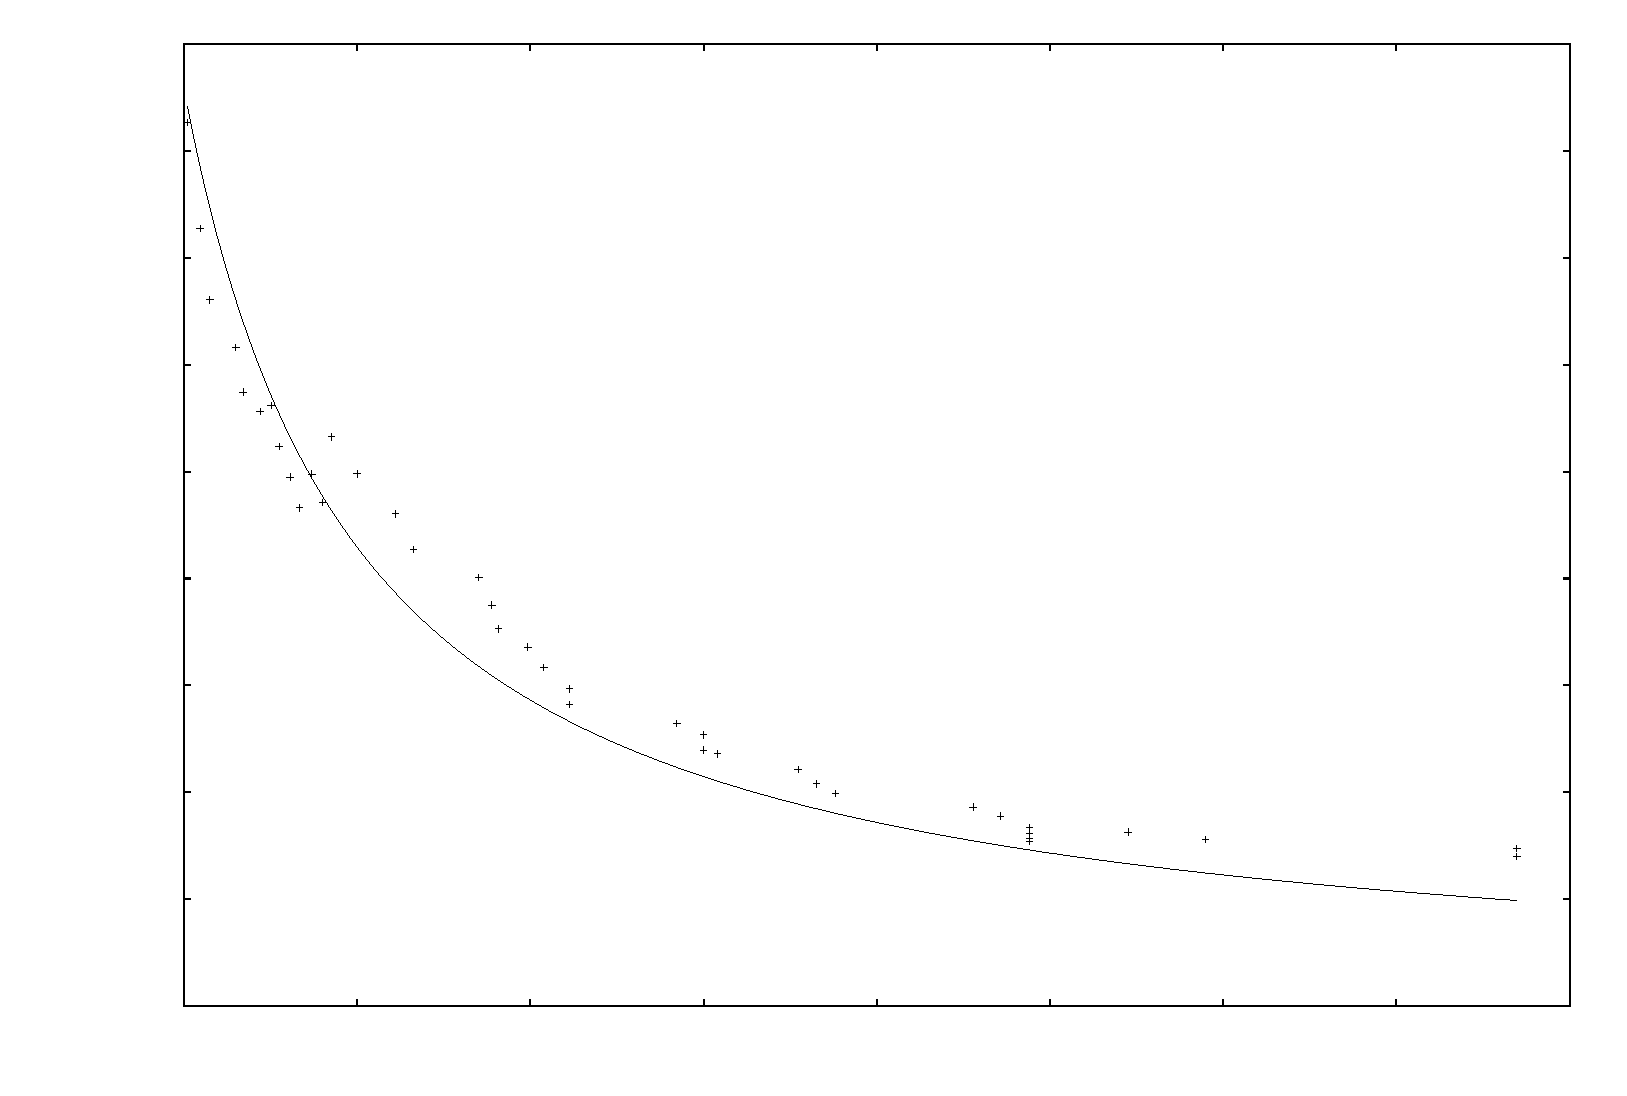
\includegraphics{plot-data-9}}%
    \gplfronttext
  \end{picture}%
\endgroup

\end{landscape}

\end{document}
